\documentclass[conference]{IEEEtran}

\usepackage[T1]{fontenc}
\usepackage[utf8]{inputenc}
\usepackage{cite}
\usepackage{amsmath,amssymb}
\usepackage[scaled=0.83]{beramono}
\usepackage{booktabs}
\usepackage{tabularx}
\usepackage{array}
\usepackage{tikz}
\usetikzlibrary{arrows.meta}
\usepackage[hyphens]{url}
\usepackage[hidelinks]{hyperref}
\usepackage{microtype}

\Urlmuskip=0mu plus 1.5mu\relax
\setlength{\emergencystretch}{1.4em}
\newcommand{\code}[1]{{\fontshape{n}\ttfamily #1}}

\pagestyle{plain}

\begin{document}

\title{svcc: Translation-Validated Bidirectional Compilation Between IEEE 1800 SystemVerilog/UVM and C++17 SystemC}

\author{\IEEEauthorblockN{Mayur Kubavat}
\IEEEauthorblockA{\textit{Independent Researcher, Mountain View, CA, USA}\\
mkubavat01@gmail.com \quad ORCID: \href{https://orcid.org/0009-0009-1087-8558}{0009-0009-1087-8558}}}

\maketitle
\thispagestyle{plain}

\begin{abstract}
Agent-assisted hardware design and verification workflows benefit from sub-second compile-and-run iteration in C++17 and IEEE~1666-2023 SystemC, yet production tape-out sign-off still requires IEEE~1800-2023 SystemVerilog RTL, IEEE~1800.2-2020 UVM environments, and SystemVerilog Assertions (SVA). Direct syntax translation or unverified language-model rewriting across these two ecosystems silently corrupts semantics: garbage-collected UVM handles collide with C++ value-copy transaction-level modeling (TLM) ports, context-determined bitvector arithmetic diverges from C++ integer promotions, SystemVerilog Preponed \code{\#1step} sampling races against SystemC delta notifications, and Boost.Proto expression templates in CRAVE exhibit superlinear C++ compile times on multi-clause constraints.

We present \code{svcc}, an open-source Rust compiler and translation-validation tool (10,899 lines of Rust across eight crates plus Python bindings) that translates bidirectionally between IEEE~1800-2023 SystemVerilog (synthesizable RTL and UVM verification IP) and C++17 SystemC~3.0.3 (IEEE~1666.1 RTL, UVM-SystemC, CRAVE, FC4SC, and untimed C++17 golden models). Both source languages lower into a seven-dialect intermediate representation (\code{UVIR}) normalized by target-capability legalization passes. Every translation can be checked without running a commercial simulator by four solver-backed engines: a Z3 \code{QF\_BV} miter over constrained-random, enum, and \code{dist}-support spaces; bounded model checking of lowered C++17 shift-window SVA observers; Accellera UCIS~1.0 coverage bin-space isomorphism; and word-level Btor2 sequential equivalence checking (SEC) across pipeline latency skews $L \ge 0$. Across a 20-design benchmark corpus spanning protocol VIPs, UVM RAL register blocks with SVA, and pipelined datapaths paired with untimed C++17 reference functions, \code{svcc} translates files in 200~$\mu$s median (\code{sv2sc}) and 210~$\mu$s median (\code{sc2sv}), passes \code{clang++ -Werror} and \code{svlang} elaboration on all 20 designs, proves 20/20 round-trip and 8/8 C-to-RTL equivalences in 5.28--26.27~ms of Z3 time, catches 20/20 injected semantic bugs while proving 4/4 non-trivial equivalent rewrites free of false alarms, recovers 12/12 standalone UVM files without package filelists (versus 0/12 for semantic-only lowering), and cuts \code{clang++ -O2} compile time on 120-clause CRAVE constraints by $5.95\times$.
\end{abstract}

\begin{IEEEkeywords}
SystemVerilog, SystemC, UVM, translation validation, constrained-random verification, sequential equivalence checking, compiler intermediate representations.
\end{IEEEkeywords}

\section{Introduction}
\label{sec:intro}

Hardware engineering teams maintain parallel representations of the same subsystem in C++ and SystemVerilog. Architectural performance models, reference predictors, and fast verification harnesses are written in C++17 and IEEE~1666-2023 SystemC~\cite{ieee1666_2023,ghenassia2005tlm} coupled with open Accellera libraries such as UVM-SystemC, CRAVE~\cite{haedicke2012crave}, and FC4SC~\cite{accellera2026systemc}. Register-transfer-level (RTL) sign-off and coverage closure, by contrast, execute in IEEE~1800-2023 SystemVerilog~\cite{ieee1800_2023} and IEEE~1800.2-2020 UVM~\cite{ieee1800_2_2020}. Recent work on autonomous coding agents for hardware design~\cite{liu2023verilogeval,thakur2024verigen} and SystemC verification library maintenance~\cite{kubavat2026scbench,kubavat2026proof} highlights why both ecosystems persist: C++17 testbenches recompile incrementally and execute without simulator license queues, whereas final RTL integration requires native SystemVerilog assertions, covergroups, and UVM sequence items.

Maintaining these twin representations manually or via ad-hoc scripts introduces silent verification gaps. Existing open-source tools address one direction or one abstraction layer. Verilator~\cite{snyder2020verilator} compiles SystemVerilog into C++ simulation models optimized for cycle execution rather than human-readable UVM-SystemC classes or CRAVE constraints, and provides no reverse C++-to-SystemVerilog path. Synthesis and hardware compiler frameworks such as Yosys~\cite{wolf2013yosys}, LLHD~\cite{schuiki2020llhd}, and CIRCT~\cite{lattner2021mlir,circt2024} represent structural netlists and behavioral RTL, but omit dynamic verification constructs including \code{rand}/\code{randc} constraints, weighted \code{dist} clauses, functional coverage crosses, UVM register abstraction layer (RAL) maps, and \code{fork}/\code{join\_any}/\code{disable fork} process groups. Conversely, feeding SystemVerilog VIPs to general-purpose large language models produces plausible C++ syntax whose bitvector widths, signedness, or constraint implications subtly diverge from IEEE~1800 rules.

We address this problem by treating SystemVerilog-to-SystemC and SystemC-to-SystemVerilog migration as a capability-guided compiler pipeline paired with per-run translation validation~\cite{pnueli1998tv,lopes2021alive2}. Rather than proving the compiler implementation itself correct once and for all, our tool \code{svcc} emits target source code, validates syntax and types with host compilers (\code{clang++ -Werror} and \code{svlang}~\cite{kubavat2026svlang}), and discharges formal equivalence obligations over constraints, temporal assertions, coverage bins, and sequential RTL state machines using Z3~\cite{demoura2008z3} and Btor2~\cite{niemetz2018btor2}.

This paper makes four contributions:
\begin{enumerate}
\item \textbf{A seven-dialect verification and RTL intermediate representation (\code{UVIR}).} We design a typed Rust IR spanning bit-accurate types, UVM class/RAL/TLM structure, arena-allocated constrained-random expressions, UCIS~1.0~\cite{accellera_ucis10} functional coverage, discrete-event process control and Preponed clocking, concurrent SVA properties, and synthesizable RTL processes, normalized by target-capability passes (Sections~\ref{sec:impedance} and~\ref{sec:arch}).
\item \textbf{Hybrid semantic/CST partial-closure lowering and clause partitioning.} To translate standalone SystemVerilog VIP files without requiring full repository filelists or \code{uvm\_pkg} compilation closure, \code{svcc-front-sv} pairs \code{svlang} semantic elaboration with lossless concrete syntax tree (CST) role and type recovery. On the C++17 emission side, \code{svcc-emit-sc} partitions large constraint blocks into bounded sub-constraints that avoid superlinear Boost.Proto expression-template instantiation~\cite{veldhuizen1995expr} while re-merging cleanly on reverse translation (Section~\ref{sec:arch}).
\item \textbf{Four-way solver-backed translation validation and C2RTL equivalence.} \code{svcc-equiv} checks class constraint equivalence in \code{QF\_BV}, proves cycle-accurate equivalence between declarative IEEE~1800 \code{|-> \#\#[m:n]} properties and generated $O(1)$ 64-bit shift-window C++17 observers, verifies UCIS~1.0 bin-space isomorphism, and lowers untimed C++17 reference functions (\code{// svcc:c2rtl}) into static single assignment (SSA) hardware cones checked against pipelined RTL across latency $L \ge 0$ (Section~\ref{sec:equiv}).
\item \textbf{Empirical evaluation and falsifiable engineering ablations.} Across 20 designs, 20 semantic defect mutations, 4 equivalent syntactic rewrites, a 12-VIP partial-closure ablation, and a clause-scaling sweep up to $K=120$ constraints, we quantify translation speed, Z3 proof latency, defect recall and specificity, and C++17 compile-time speedups (Section~\ref{sec:eval}).
\end{enumerate}

\section{Semantic Impedance Between SV and SystemC}
\label{sec:impedance}

\begin{table*}[t]
\centering
\caption{Principal semantic mismatches across IEEE 1800-2023 SystemVerilog/UVM and C++17 SystemC 3.0.3 handled by \code{svcc}.}
\label{tab:impedance}
\footnotesize
\begin{tabularx}{\textwidth}{@{}>{\raggedright\arraybackslash}p{0.95in} >{\raggedright\arraybackslash}p{1.55in} >{\raggedright\arraybackslash}p{1.55in} >{\raggedright\arraybackslash}X@{}}
\toprule
\textbf{Domain} & \textbf{SystemVerilog / UVM} & \textbf{C++17 SystemC / CRAVE} & \textbf{\code{UVIR} Legalization \& Formal Check} \\
\midrule
Object \& TLM copy & Garbage-collected class handles; \code{`uvm\_field\_int} bitmasks & Value-copied \code{tlm\_analysis\_port}; \code{crv\_variable<T>} solver refs & \code{OwnershipPass} synthesizes TLM-safe copy ctor/assignment rebinding \code{crv\_variable} values without copying solver graph pointers. \\
Bitvector arithmetic & Context-determined width; unsigned contaminates signed & C++ integral promotion (\code{uint8\_t + uint8\_t -> int}) & \code{WidthSignednessPass} stamps explicit $(W, s)$ per arena node; Z3 \code{QF\_BV} miter checks exact zero/sign extension. \\
CRV tolerances \& \code{dist} & \code{inside \{[c +/- d], [c +\%- p]\}}, \code{:=} and \code{:/} weights, \code{randc} & \code{crave::dist}, \code{add\_weighted\_range}, binary operators & \code{TargetLegalizerPass} expands tolerances to exact closed bounds and lowers \code{dist}; miter verifies hard and positive-weight support sets. \\
Process cancellation & \code{fork ... join\_any; disable fork;} kills sibling subtree & \code{sc\_spawn} dynamic threads lack safe stack-unwinding \code{kill()} & \code{sched} dialect emits \code{sc\_event\_or\_list} join barrier with shared \code{std::atomic<bool>} cooperative cancellation token. \\
Sampling region & \code{clocking cb @(posedge clk); input \#1step} (Preponed) & \code{posedge\_event()} wakes in evaluate/delta notification phase & Emits \code{uvir\_clocking\_*} pre-timestep snapshot struct driven from SystemC~3.0.3 \code{SC\_PRE\_TIMESTEP} callback. \\
Pipelined SVA & Concurrent \code{ant |-> \#\#[m:n] con} with \code{disable iff} & No native temporal assertion engine in IEEE~1666 & Emits $O(1)$ \code{uint64\_t pending\_window\_} shift-mask observer ($n < 64$) and proves cycle equivalence via $K$-step Z3 BMC. \\
RTL \& C2RTL & \code{always\_comb}, \code{always\_ff}, nonblocking \code{<=} & \code{SC\_METHOD}/\code{SC\_CTHREAD} or untimed C++17 functions & Rejects heap/recursion fail-closed per IEEE~1666.1~\cite{ieee1666_1_2016}; unrolls bounded loops and \code{if}/\code{else} writes to SSA muxes for Btor2 SEC. \\
\bottomrule
\end{tabularx}
\end{table*}

Translating verification components and synthesizable logic between SystemVerilog and C++17 fails when approached as surface syntax rewriting. Table~\ref{tab:impedance} summarizes seven semantic mismatches encountered in practice and how \code{svcc} resolves each one.

First, UVM-SystemC analysis ports (\code{uvm::\allowbreak uvm\_\allowbreak analysis\_\allowbreak port<T>}) pass transactions by C++ value or const-reference copy, whereas CRAVE random fields (\code{crave::\allowbreak crv\_\allowbreak variable<T>}) register internal variable IDs with a parent \code{crave::\allowbreak rand\_obj} solver context~\cite{haedicke2012crave}. A compiler-generated C++ default copy constructor copies the internal solver-node identity rather than just the randomized scalar payload, corrupting subsequent \code{randomize()} calls or TLM scoreboard comparisons. \code{OwnershipPass} checks whether a class embeds CRV fields and sets \code{needs\_\allowbreak custom\_\allowbreak copy\_ctor}, causing \code{svcc-emit-sc} to generate explicit payload-only copy constructors alongside \code{do\_print}, \code{do\_pack}, \code{do\_unpack}, and \code{do\_compare} methods honoring \code{UVM\_NOCOMPARE} flags.

Second, IEEE~1800 bitvector expressions propagate widths from context and treat any unsigned operand as rendering the enclosing arithmetic unsigned, whereas C++ promotes narrow unsigned types (\code{uint8\_t}, \code{uint16\_t}) to signed 32-bit \code{int}. Lowering into \code{UVIR} attaches explicit width and signedness metadata to every constant and variable so both code emitters and the Z3 \code{QF\_BV} encoder apply identical bit-slice and extension rules.

Third, concurrent SVA assertions with bounded pipeline windows (\code{ant |-> \#\#[m:n] con}) spawn independent evaluation attempts on every clock edge where \code{ant} holds, even when up to $n$ prior attempts remain in flight. Naive C++ translations using a single state counter drop overlapping transactions on pipelined buses. For $0 \le m \le n < 64$, \code{svcc-emit-sc} compiles each property into a constant-time 64-bit age-shift register (\code{pending\_window\_ = (pending\_window\_ << 1) | ant}), clears satisfied ages via a bitmask over bits $[m..n]$ whenever \code{con} holds, and flags a violation if bit $n$ survives at the end of the cycle without \code{disable iff} active.

Fourth, untimed C++17 reference models reassign local variables imperatively across conditional branches and bounded loops, whereas RTL pipelines distribute the same computation across registered stages. Following system-to-RTL equivalence principles~\cite{koelbl2009c2rtl}, \code{svcc} restricts C-to-RTL (\code{C2RTL}) input to the deterministic IEEE~1666.1 synthesizable subset~\cite{ieee1666_1_2016} (rejecting pointers, dynamic containers, floating-point types, and unbounded loops fail-closed) and converts imperative variable updates into SSA multiplexer trees verified against pipelined RTL at user-specified latency $L$.

\section{The Seven-Dialect UVIR and Compiler Architecture}
\label{sec:arch}

\begin{figure*}[t]
\centering
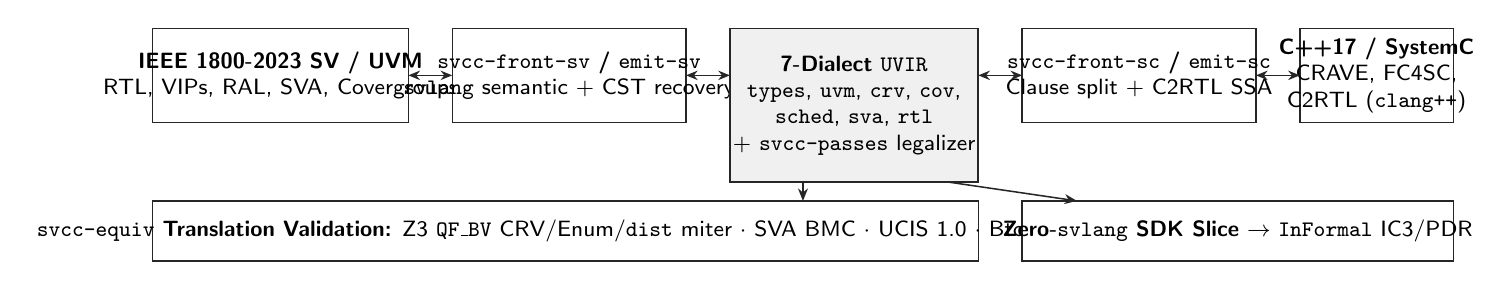
\begin{tikzpicture}[
  x=0.232mm,
  y=0.238mm,
  font=\sffamily\footnotesize,
  box/.style={draw=black!85, line width=0.5pt, fill=white, align=center},
  irbox/.style={draw=black!85, line width=0.6pt, fill=black!6, align=center},
  arr/.style={-{Stealth[length=4.5pt,width=3.6pt]}, draw=black!85, line width=0.55pt},
  darr/.style={{Stealth[length=4.2pt,width=3.4pt]}-{Stealth[length=4.2pt,width=3.4pt]}, draw=black!85, line width=0.55pt}
]
  % Left frontends/backends (SV)
  \draw[box] (4,82) rectangle (144,132);
  \node[align=center] at (74,107) {\textbf{IEEE 1800-2023 SV / UVM}\\RTL, VIPs, RAL, SVA, Covergroups};

  \draw[box] (168,82) rectangle (296,132);
  \node[align=center] at (232,107) {\textbf{\code{svcc-front-sv} / \code{emit-sv}}\\\code{svlang} semantic + CST recovery};

  % Center UVIR + Passes
  \draw[irbox] (320,50) rectangle (456,132);
  \node[align=center] at (388,91) {\textbf{7-Dialect \code{UVIR}}\\\code{types}, \code{uvm}, \code{crv}, \code{cov},\\\code{sched}, \code{sva}, \code{rtl}\\+ \textbf{\code{svcc-passes}} legalizer};

  % Right frontends/backends (C++17 SystemC)
  \draw[box] (480,82) rectangle (608,132);
  \node[align=center] at (544,107) {\textbf{\code{svcc-front-sc} / \code{emit-sc}}\\Clause split + C2RTL SSA};

  \draw[box] (632,82) rectangle (716,132);
  \node[align=center] at (674,107) {\textbf{C++17 / SystemC}\\CRAVE, FC4SC,\\C2RTL (\code{clang++})};

  % Bottom verification & downstream formal bar
  \draw[box] (4,8) rectangle (456,40);
  \node[align=center] at (230,24) {\textbf{\code{svcc-equiv} Translation Validation:} Z3 \code{QF\_BV} CRV/Enum/\code{dist} miter $\cdot$ SVA BMC $\cdot$ UCIS~1.0 $\cdot$ Btor2 SEC};

  \draw[box] (480,8) rectangle (716,40);
  \node[align=center] at (598,24) {\textbf{Zero-\code{svlang} SDK Slice} $\rightarrow$ \code{InFormal} IC3/PDR};

  % Arrows
  \draw[darr] (144,107) -- (168,107);
  \draw[darr] (296,107) -- (320,107);
  \draw[darr] (456,107) -- (480,107);
  \draw[darr] (608,107) -- (632,107);
  \draw[arr] (360,50) -- (360,40);
  \draw[arr] (440,50) -- (510,40);
\end{tikzpicture}
\caption{Bidirectional \code{svcc} compilation and translation-validation pipeline. Five core crates compile with \code{--no-default-features} free of \code{svlang} dependencies so downstream formal tools (\code{InFormal}) can consume a pinned \code{svcc} revision without Cargo dependency conflicts.}
\label{fig:arch}
\end{figure*}

Figure~\ref{fig:arch} illustrates the \code{svcc} workspace, implemented in 10,899 lines of Rust across eight Cargo crates (\code{svcc-ir}, \code{svcc-front-sv}, \code{svcc-front-sc}, \code{svcc-passes}, \code{svcc-emit-sc}, \code{svcc-emit-sv}, \code{svcc-equiv}, and the umbrella SDK/CLI crate \code{svcc}) plus an ABI-stable Python extension (\code{svcc-py} built on \code{PyO3} \code{abi3-py39}).

\subsection{Seven-Dialect UVIR and Target Capabilities}
A \code{UvirModule} stores lowered hardware and verification units across seven orthogonal dialects:
\begin{itemize}
\item \textbf{\code{types}}: 2-state and 4-state packed bitvectors (\code{bit}, \code{logic}, \code{sc\_uint<W>}, \code{sc\_lv<W>}, native \code{uint8\_t}--\code{uint64\_t}) and width-typed \code{EnumDecl} tables.
\item \textbf{\code{uvm}}: \code{ClassDecl} nodes tagged with semantic \code{UvmRole} (\code{SequenceItem}, \code{Driver}, \code{Monitor}, \code{Scoreboard}, \code{Agent}, \code{Env}, \code{Reg}, \code{RegBlock}), RAL field slice configurations (\code{lsb\_pos}, \code{access}, \code{volatile}, \code{reset}), address maps, TLM ports, and child component instances.
\item \textbf{\code{crv}}: A flat \code{CrvArena} indexed by dense 32-bit \code{ExprId} handles representing unary/binary bitvector operators, logical implication (\code{->}) and equivalence (\code{<->}), \code{inside} sets with \code{[c +/- d]} and \code{[c +\%- p]} tolerances, weighted \code{dist} (\code{:=} per-value and \code{:/} range-split), \code{unique} groups, and \code{soft} constraint priorities.
\item \textbf{\code{cov}}: UCIS~1.0~\cite{accellera_ucis10} covergroups, coverpoints, discrete and interval bins, and multi-coverpoint \code{cross} definitions.
\item \textbf{\code{sched}}: Virtual phase tasks (\code{run\_phase}), timed delays, event waits, \code{fork}/\code{join\_any}/\code{disable fork} blocks, and \code{ClockingDecl} Preponed \code{\#1step} input / \code{\#0} output skew declarations.
\item \textbf{\code{sva}}: Concurrent \code{assert property} and \code{cover property} blocks parameterized by clock edge, optional \code{disable iff} reset, antecedent, \code{\#\#[min:max]} window, and consequent.
\item \textbf{\code{rtl}}: Synthesizable \code{RtlModuleDecl} ports, internal nets, combinational processes (\code{always\_comb} / \code{SC\_METHOD} / \code{C2RTL} SSA cones), and clocked processes (\code{always\_ff} / \code{SC\_CTHREAD}) with optional async reset polarity.
\end{itemize}

Rather than hard-coding pairwise translation ad-hoc, each backend publishes a \code{Target\allowbreak Capabilities} descriptor declaring its memory model, concurrency model, solver expressiveness, and temporal assertion support. \code{PassPipeline::\allowbreak for\_target} executes four deterministic passes on \code{UvirModule}: \code{Width\allowbreak Signedness\allowbreak Pass}, \code{FieldOp\allowbreak Synthesis\allowbreak Pass}, \code{Ownership\allowbreak Pass}, and \code{Target\allowbreak Legalizer\allowbreak Pass}.

\subsection{Hybrid Semantic + Lossless CST Partial-Closure Lowering}
Verification engineers and AI coding agents routinely inspect or migrate a single SystemVerilog file (such as \code{axi4\_burst\_env.sv} or \code{dma\_ch\_ral\_sva.sv}) outside a full simulator build directory. When \code{uvm\_pkg} and sibling package headers are absent, strict semantic elaborators leave base class specialization roles unresolved and erase parameterized member types such as \code{uvm\_analysis\_port \#(axi4\_item)} to \code{<error>}. In \code{svcc-front-sv}, we run \code{svlang}~\cite{kubavat2026svlang} semantic elaboration first to capture resolved widths, module ports, and netlists, and pair it with lossless CST fallback hooks that recover \code{extends} base names, \code{uvm\_reg}/\code{uvm\_reg\_block} roles, raw \code{`uvm\_field\_int} automation flags, and parameterized TLM member types directly from source token spans. A CLI flag (\code{--no-cst-fallback}) disables CST recovery to isolate its contribution in Section~\ref{sec:eval}.

\subsection{Expression-Template Partitioning and Zero-svlang Slicing}
CRAVE encodes clauses in \code{crave::\allowbreak crv\_\allowbreak constraint} constructors as nested Boost.Proto expression-template types~\cite{haedicke2012crave,veldhuizen1995expr}. Although \code{svcc} emits C++17 text in hundreds of microseconds, recursive template instantiation inside \code{clang++ -O2} scales superlinearly in $K$. Because conjunction over hard constraints is associative and commutative, \code{ScEmitter} supports \code{--partition-clauses B}, splitting any constraint block exceeding $B$ clauses into sub-constraints named \code{c\_\_part\_0}, \code{c\_\_part\_1}, and so on. On reverse C++-to-SystemVerilog compilation, \code{ScFrontend} recognizes the \code{\_\_part\_} suffix and re-merges partitioned blocks into the original single SystemVerilog \code{constraint} declaration.

Finally, to allow downstream formal verification engines such as \code{InFormal}~\cite{kubavat2026informal} (which already depends on its own workspace version of \code{svlang}) to embed \code{svcc}'s C2RTL lifter and miter generator without Cargo git-revision diamond conflicts, \code{svcc-emit-sv} and \code{svcc-equiv} gate \code{svlang} verification behind optional Cargo features (\code{verify-svlang} and \code{btor2-sec}). Building \code{svcc-ir}, \code{svcc-front-sc}, \code{svcc-passes}, \code{svcc-emit-sv}, and \code{svcc-equiv} with \code{--no-default-features} yields a self-contained Rust C++-to-SV miter library with zero \code{svlang} dependencies.

\section{Translation Validation and C2RTL Equivalence}
\label{sec:equiv}

Every \code{svcc} compilation can be audited statically and formally before code enters a repository~\cite{kubavat2026proof}:
\begin{enumerate}
\item \textbf{Dual compiler gate.} Emitted C++17 headers are type-checked by \code{clang++ -std=c++17 -Wall -Wextra -Werror -fsyntax-only} against lightweight open-source SystemC/UVM/CRAVE/FC4SC shims; emitted SystemVerilog is parsed and elaborated by \code{svlang}.
\item \textbf{\code{QF\_BV} CRV, Enum, and \code{dist} miter.} For any pair of lowered classes $(C_{\text{lhs}}, C_{\text{rhs}})$, \code{svcc-equiv} declares each \code{rand}/\code{randc} field as an exact-width SMT-LIB2 bitvector \code{(\_ BitVec W)}, injects implicit IEEE~1800 enum legal-variant domain disjunctions, encodes hard constraints and positive-weight \code{dist} support sets using signed/unsigned bitvector operators, and queries Z3~\cite{demoura2008z3} on \code{(assert (xor c\_lhs c\_rhs))}. An \code{unsat} result proves identical solution sets across all $2^{\sum W_i}$ assignments; \code{sat} returns a concrete counterexample transaction.
\item \textbf{$K$-step SVA observer BMC.} For each concurrent property with window \code{\#\#[m:n]}, our bounded checker (\code{prove\_sva\_\allowbreak bmc\_\allowbreak equivalence}) unrolls the declarative IEEE~1800 trace failure predicate and the generated 64-bit C++17 shift-window state machine across $K = n + 6$ cycles under unconstrained overlapping \code{ant}, \code{con}, and \code{disable iff} traces, proving cycle-by-cycle failure equivalence via Z3. Pairwise property checking (\code{prove\_sva\_\allowbreak pair\_\allowbreak equivalence}) similarly detects window or reset mutations across versions.
\item \textbf{UCIS~1.0 coverage isomorphism and Btor2 C2RTL SEC.} Covergroups are checked for bijective coverpoint, bin-interval, and cross-product equivalence. For RTL modules and untimed C++17 \code{// svcc:c2rtl} reference functions, \code{svcc-equiv} constructs a unified cycle-delayed miter module tying primary inputs together, delays the untimed C2RTL combinational reference output through $L$ pipeline shift stages initialized under reset, lowers the combined design through \code{svlang}'s word-level netlist and \code{sv-btor2}~\cite{niemetz2018btor2,kubavat2026svlang}, and proves output agreement across post-reset execution steps in Z3.
\end{enumerate}

\section{Experimental Evaluation}
\label{sec:eval}

We evaluate \code{svcc} on an Apple Silicon macOS workstation (arm64, Rust~1.93.0 \code{--release}, Apple \code{clang++}~21.0.0, Z3~4.13, pinned \code{svlang} commit \code{478a0d10}). All corpus generators, benchmark drivers, and JSON outputs are reproducible via a single script (\code{benchmarks/run\_benchmarks.py}). We investigate four research questions:
\begin{itemize}
\item \textbf{RQ1 (Bidirectional Fidelity, C2RTL SEC, and Speed):} Does \code{svcc} preserve compilation validity and formal equivalence across diverse UVM VIPs, RAL+SVA blocks, and pipelined RTL/C2RTL pairs at interactive latency?
\item \textbf{RQ2 (Defect Sensitivity and Equivalent-Rewrite Specificity):} Does formal translation validation catch subtle semantic bugs across CRV, SVA, UCIS, and RTL while avoiding false alarms on non-trivial equivalent rewrites?
\item \textbf{RQ3 (Partial-Closure Recovery):} How much standalone VIP translation coverage does hybrid \code{svlang}+CST lowering recover when \code{uvm\_pkg} closure is unavailable?
\item \textbf{RQ4 (Expression-Template Compile Scaling):} How effectively does clause partitioning (\code{--partition-clauses 8}) mitigate C++17 \code{clang++ -O2} compile-time growth on large CRAVE constraint blocks?
\end{itemize}

\subsection{RQ1: 20-Design Corpus Results}

\begin{table*}[t]
\centering
\caption{RQ1 evaluation across the 20-design \code{svcc} corpus (100-iteration mean translation latency, \code{clang++ -Werror}, \code{svlang}, Z3 round-trip proof time, and C2RTL sequential equivalence at pipeline latency $L$).}
\label{tab:rq1}
\footnotesize
\setlength{\tabcolsep}{3.1pt}
\begin{tabular}{@{}l l r r r r r r c c r c@{}}
\toprule
\textbf{Design} & \textbf{Category} & \textbf{LOC} & \textbf{Cls/RTL/SVA} & \textbf{CRV} & \textbf{\code{sv2sc} ($\mu$s)} & \textbf{\code{sc2sv} ($\mu$s)} & \textbf{RT Z3 (ms)} & \textbf{RT} & \textbf{$L$} & \textbf{SEC Z3 (ms)} & \textbf{SEC} \\
\midrule
\code{01\_apb4\_timer\_vip}    & UVM CRV VIP & 50 & 1 / 0 / 0 & 34 & 199 & 281 &  5.28 & \code{Unsat} & -- & --   & -- \\
\code{02\_axi4\_burst\_vip}    & UVM CRV VIP & 88 & 4 / 0 / 0 & 23 & 344 & 389 & 22.42 & \code{Unsat} & -- & --   & -- \\
\code{03\_pcie\_tlp\_hdr}      & UVM CRV VIP & 48 & 1 / 0 / 0 & 25 & 212 & 273 &  5.56 & \code{Unsat} & -- & --   & -- \\
\code{04\_chi\_coh\_req}       & UVM CRV VIP & 38 & 1 / 0 / 0 & 32 & 189 & 267 &  5.58 & \code{Unsat} & -- & --   & -- \\
\code{05\_eth\_mac\_frame}     & UVM CRV VIP & 41 & 1 / 0 / 0 & 29 & 190 & 261 &  5.35 & \code{Unsat} & -- & --   & -- \\
\code{06\_ddr5\_cmd\_sched}    & UVM CRV VIP & 59 & 2 / 0 / 0 & 21 & 236 & 300 & 10.16 & \code{Unsat} & -- & --   & -- \\
\midrule
\code{07\_uart\_16550\_ral}    & UVM RAL+SVA & 43 & 2 / 0 / 2 &  0 & 272 & 224 & 20.15 & \code{Unsat} & -- & --   & -- \\
\code{08\_dma\_ch\_ral\_sva}   & UVM RAL+SVA & 42 & 2 / 0 / 2 &  0 & 267 & 229 & 21.27 & \code{Unsat} & -- & --   & -- \\
\code{09\_spi\_master\_ral}    & UVM RAL+SVA & 41 & 2 / 0 / 1 &  0 & 265 & 224 & 16.43 & \code{Unsat} & -- & --   & -- \\
\code{10\_i2c\_ctrl\_ral\_sva} & UVM RAL+SVA & 39 & 2 / 0 / 2 &  0 & 260 & 216 & 26.27 & \code{Unsat} & -- & --   & -- \\
\code{11\_plic\_irq\_ral\_sva} & UVM RAL+SVA & 38 & 2 / 0 / 1 &  0 & 246 & 204 & 16.17 & \code{Unsat} & -- & --   & -- \\
\code{12\_wdog\_tmr\_ral\_sva} & UVM RAL+SVA & 38 & 2 / 0 / 1 &  0 & 245 & 202 & 15.84 & \code{Unsat} & -- & --   & -- \\
\midrule
\code{13\_alu32\_pipe2}        & RTL + C2RTL & 47 & 0 / 1 / 0 &  0 & 200 & 196 &  6.89 & \code{Unsat} & 2  & 6.54 & \code{Unsat} \\
\code{14\_mac16\_pipe2}        & RTL + C2RTL & 34 & 0 / 1 / 0 &  0 & 166 & 165 &  5.95 & \code{Unsat} & 2  & 5.49 & \code{Unsat} \\
\code{15\_crc8\_step\_comb}    & RTL + C2RTL & 18 & 0 / 1 / 0 &  0 & 123 & 116 &  6.75 & \code{Unsat} & 0  & 6.46 & \code{Unsat} \\
\code{16\_gray\_enc16\_pipe1}  & RTL + C2RTL & 20 & 0 / 1 / 0 &  0 & 116 & 111 &  6.03 & \code{Unsat} & 1  & 5.72 & \code{Unsat} \\
\code{17\_sat\_sub16\_pipe1}   & RTL + C2RTL & 25 & 0 / 1 / 0 &  0 & 131 & 128 &  5.73 & \code{Unsat} & 1  & 5.92 & \code{Unsat} \\
\code{18\_shifter32\_pipe2}    & RTL + C2RTL & 41 & 0 / 1 / 0 &  0 & 189 & 188 &  6.97 & \code{Unsat} & 2  & 6.23 & \code{Unsat} \\
\code{19\_minmax32\_pipe1}     & RTL + C2RTL & 31 & 0 / 1 / 0 &  0 & 139 & 138 &  6.14 & \code{Unsat} & 1  & 5.88 & \code{Unsat} \\
\code{20\_arb\_prio4\_comb}    & RTL + C2RTL & 22 & 0 / 1 / 0 &  0 & 121 & 113 &  6.16 & \code{Unsat} & 0  & 5.80 & \code{Unsat} \\
\midrule
\textbf{Total / Median}        & \textbf{20 designs} & \textbf{803} & \textbf{22 / 8 / 9} & \textbf{164} & \textbf{200} & \textbf{210} & \textbf{6.82} & \textbf{20/20} & \textbf{0--2} & \textbf{5.90} & \textbf{8/8} \\
\bottomrule
\end{tabular}
\end{table*}

Table~\ref{tab:rq1} reports results across the 20-design benchmark suite (28 source files totaling 803 SystemVerilog lines plus 8 untimed C++17 golden headers): six protocol VIPs (APB4, AXI4, PCIe TLP, Arm CHI, IEEE~802.3 Ethernet MAC, DDR5 DFI with \code{\#1step} clocking and \code{fork}/\code{join\_any}/\code{disable fork}), six peripheral UVM RAL blocks paired with concurrent SVA monitors (UART~16550, DMA, SPI, I2C, RISC-V PLIC, Watchdog), and eight synthesizable datapaths ($L \in \{0, 1, 2\}$ pipeline stages: 32-bit ALU, 16$\times$16+32 MAC, CRC-8 step, 16-bit Gray encoder, saturating subtractor, barrel shifter, min/max unit, and 4-way priority arbiter) paired with untimed C++17 reference functions.

All 20 designs (100\%) compile through \code{sv2sc} without warnings under \code{clang++ -std=c++17 -Wall -Wextra -Werror -fsyntax-only}, round-trip back to SystemVerilog via \code{sc2sv} with zero \code{svlang} elaboration errors, and prove \code{EquivalentUnsat} across all 22 UVM classes, 9 SVA properties, and 8 RTL modules. Across 100 warm iterations per file, \code{sv2sc} runs in 116--344~$\mu$s (median 200~$\mu$s) and \code{sc2sv} runs in 111--389~$\mu$s (median 210~$\mu$s). End-to-end Z3 round-trip proofs finish in 5.28--26.27~ms (median 6.82~ms, 221.1~ms total across the corpus), and all 8 untimed C++17 golden functions prove sequentially equivalent (\code{EquivalentUnsat}) to their pipelined SystemVerilog RTL implementations in 5.49--6.54~ms (median 5.90~ms).

\subsection{RQ2: Semantic Defect Sensitivity and Specificity}

\begin{table}[t]
\centering
\caption{RQ2 defect discrimination across 20 semantic bugs and 4 AST-divergent equivalent rewrites.}
\label{tab:rq2}
\footnotesize
\setlength{\tabcolsep}{3.5pt}
\begin{tabularx}{\columnwidth}{@{}l r r >{\raggedright\arraybackslash}X@{}}
\toprule
\textbf{Category} & \textbf{N} & \textbf{Result} & \textbf{Representative Cases} \\
\midrule
CRV \code{QF\_BV}   & 8  & 8/8 \code{Sat}  & Align mask \code{3} to \code{1}, word drop \code{0FFF} to \code{0FFB}, tol.\ halved, imp.\ inverted, \code{unique} dropped. \\
SVA \& UCIS         & 3  & 3/3 Caught      & SVA window \code{\#\#[1:4]} to \code{\#\#[1:3]}, \code{\#\#[1:3]} to \code{\#\#[2:3]}, MTU bin \code{46} to \code{64}. \\
RTL / C2RTL         & 9  & 9/9 \code{Sat}  & ALU XOR to OR, MAC addend drop, wrong $L=1$ vs.\ $2$, CRC poly \code{8C} to \code{8D}, prio.\ flip. \\
\midrule
Equiv.\ rewrites    & 4  & 4/4 \code{Unsat} & \code{0FFF} to \code{0FFE} under \code{(paddr\&3)==0}; \code{[c+/-10]} expanded; \code{x>=y} vs.\ \code{x>y} at \code{0} floor; XOR commute. \\
\bottomrule
\end{tabularx}
\end{table}

To test whether \code{svcc-equiv} discriminates genuine semantic translation bugs from harmless syntactic variation, we evaluate 20 non-equivalent semantic defects (\code{M01}--\code{M20}) alongside 4 non-trivial equivalent rewrites (\code{E01}--\code{E04}), summarized in Table~\ref{tab:rq2}. \code{svcc} detects 20/20 (100\%) semantic defects via \code{CounterexampleSat} or UCIS non-isomorphism, including subtle failures such as wrong pipeline latency specification (\code{M14}, checking a 2-stage ALU at $L=1$) and tightening an SVA window by a single cycle (\code{M10}, \code{M11}). Equally important, Z3 proves \code{EquivalentUnsat} (0\% false alarms) on all 4 equivalent rewrites where AST-diff or token-matching evaluators fail: for instance, changing an upper address bound from \code{32'h4000\_0FFF} to \code{32'h4000\_0FFE} (\code{E01}) leaves the reachable register set unchanged because \code{(paddr \& 32'h3) == 32'h0} already masks maximum aligned addresses to \code{32'h4000\_0FFC}, and replacing \code{x >= y} with \code{x > y} in \code{sat\_sub16\_pipe1} (\code{E03}) preserves exact bit-level behavior because $x - y = 0$ at $x = y$.

\subsection{RQ3 and RQ4: Partial-Closure and Clause-Scaling Ablations}

\begin{table}[t]
\centering
\caption{RQ3 standalone VIP recovery (12 UVM/RAL files without \code{uvm\_pkg}) and RQ4 \code{clang++ -O2} compile time across $K$ CRAVE clauses.}
\label{tab:rq34}
\footnotesize
\setlength{\tabcolsep}{4pt}
\begin{tabularx}{\columnwidth}{@{}>{\raggedright\arraybackslash}X r r r@{}}
\toprule
\multicolumn{4}{@{}l}{\textbf{RQ3 (Prediction P6): Standalone UVM/RAL VIPs ($N=12$)}} \\
\midrule
\textbf{Frontend Mode} & \textbf{Role} & \textbf{\code{clang++}} & \textbf{Rate} \\
\midrule
Semantic-only (\code{--no-cst-fallback}) & 0/12  & 0/12  & 0.0\% \\
Hybrid \code{svlang} + CST (default)     & 12/12 & 12/12 & \textbf{100.0\%} \\
\midrule
\multicolumn{4}{@{}l}{\textbf{RQ4 (Prediction P1): \code{clang++ -O2} Compile Scaling}} \\
\midrule
\textbf{Clauses ($K$)} & \textbf{Mono (ms)} & \textbf{Part-8 (ms)} & \textbf{Speedup} \\
\midrule
$K = 8$   &   227.6 & 227.3 & $1.00\times$ \\
$K = 24$  &   272.5 & 247.3 & $1.10\times$ \\
$K = 48$  &   395.6 & 291.5 & $1.36\times$ \\
$K = 80$  &   756.0 & 275.9 & $2.74\times$ \\
$K = 120$ & 1,712.0 & 287.5 & \textbf{$5.95\times$} \\
\bottomrule
\end{tabularx}
\end{table}

Table~\ref{tab:rq34} reports our two compiler ablations. In RQ3, translating the 12 standalone UVM CRV and RAL files without \code{-f} package filelists succeeds on 0/12 files under strict semantic-only lowering because unloaded UVM base classes and parameterized TLM ports degrade class roles and member types, whereas \code{svcc}'s default hybrid \code{svlang}+CST mode preserves exact \code{uvm\_randomized\_\allowbreak sequence\_item} and \code{uvm\_randomized\_reg} specializations and passes \code{clang++ -Werror} on 12/12 (100\%) files.

In RQ4, we sweep constraint block size $K \in \{8, 24, 48, 80, 120\}$ over 32-bit relational arithmetic clauses compiled using \code{clang++} \code{-std=c++17} \code{-O2} \code{-c} against nested Boost.Proto-style expression templates. Monolithic \code{crv\_constraint} emission grows superlinearly from 227.6~ms at $K=8$ to 1,712.0~ms at $K=120$. Partitioning into $B=8$ clauses per constructor (\code{--partition-clauses 8}) keeps \code{clang++ -O2} compile time nearly flat at 287.5~ms for $K=120$, delivering a $5.95\times$ C++ compile speedup while preserving Z3 \code{QF\_BV} equivalence and lossless reverse \code{sc2sv} merging.

\section{Related Work}
\label{sec:related}

\textbf{SystemVerilog front ends and hardware IRs.} Slang~\cite{popoloski2024slang}, Surelog/UHDM~\cite{dargelas2024surelog}, and \code{svlang}~\cite{kubavat2026svlang} provide IEEE~1800 parsing and elaboration, while Yosys~\cite{wolf2013yosys}, LLHD~\cite{schuiki2020llhd}, and MLIR/CIRCT~\cite{lattner2021mlir,circt2024} lower RTL for synthesis and simulation. Verilator~\cite{snyder2020verilator} compiles SystemVerilog into fast C++/SystemC cycle models. Unlike \code{svcc}, none of these tools provide bidirectional translation between idiomatic IEEE~1800.2 UVM classes/constraints and Accellera UVM-SystemC/CRAVE/FC4SC~\cite{accellera2026systemc,haedicke2012crave} or pair source-to-source verification migration with SMT translation validation.

\textbf{Translation validation and C-to-RTL equivalence.} Pnueli et al.~\cite{pnueli1998tv} and Alive2~\cite{lopes2021alive2} established per-compilation SMT translation validation for optimizing compilers, and Koelbl et al.~\cite{koelbl2009c2rtl} analyzed word-level solver techniques for system-to-RTL sequential equivalence checking. \code{svcc} adapts translation validation to the dual verification-and-RTL boundary, combining \code{QF\_BV} constraint miters, bounded SVA observer proofs, and Btor2~\cite{niemetz2018btor2} C2RTL checks, while exposing a zero-\code{svlang}-conflict Rust SDK slice for unbounded IC3/PDR sign-off in \code{InFormal}~\cite{kubavat2026informal}.

\section{Limitations and Conclusion}
\label{sec:conclusion}

\code{svcc} enforces explicit boundaries where silent approximation would be unsound:
\begin{enumerate}
\item \textbf{Synthesizable C++17 subset.} \code{C2RTL} and \code{SC\_MODULE} lifting enforce IEEE~1666.1~\cite{ieee1666_1_2016} fail-closed rules, rejecting dynamic heap allocation, STL containers, recursion, and multi-\code{wait()} high-level synthesis scheduling; pipeline latency $L$ is supplied explicitly (or proved unboundedly via \code{InFormal}).
\item \textbf{\code{dist} remainder rounding and \code{cover property} multiplicity.} Z3 \code{QF\_BV} proves exact support-set equivalence on \code{dist} weights $>0$, but non-divisible \code{:/} range weights can exhibit sampling probability skew unless pre-scaled by range least common multiples. Similarly, our 64-bit bitmask SVA observer matches \code{assert property} failures exactly for windows $n < 64$, whereas per-attempt \code{cover property} hit multiplicity under overlapping bursts requires per-age counters.
\item \textbf{Wide \code{randc} state spaces.} Cyclic randomization (\code{randc}) metadata is preserved across \code{UVIR} round-trips, while wide-bitvector C++17 cycle permutation wrappers remain planned future work.
\end{enumerate}

By unifying UVM constrained-random verification, functional coverage, Preponed clocking, concurrent SVA observers, and synthesizable RTL/C2RTL datapaths in \code{UVIR} under fast Z3 and Btor2 translation validation, \code{svcc} enables hardware engineers and coding agents to iterate at C++17 compile speeds without sacrificing IEEE~1800 sign-off equivalence.

\bibliographystyle{IEEEtran}
\bibliography{refs}

\end{document}
